\documentclass[conference]{IEEEtran}

\IEEEoverridecommandlockouts

\usepackage{cite}
\usepackage{amsmath,amssymb,amsfonts}
\usepackage{graphicx}
\usepackage[caption=false,font=footnotesize]{subfig}
\usepackage{booktabs}
\usepackage{multirow}
\usepackage{array}
\usepackage{url}
\usepackage{xcolor}
\usepackage{hyperref}
\usepackage{tikz}
\usepackage{pgfplots}
\usepackage{algorithm}
\usepackage{algpseudocode}

\usetikzlibrary{arrows.meta,positioning,shapes.geometric,fit}
\pgfplotsset{compat=1.18}
\graphicspath{{outputs/}{test_images/}}

\hypersetup{
    colorlinks=true,
    linkcolor=blue,
    citecolor=blue,
    urlcolor=blue
}

\title{Intelligent Image Watermarking System with Predictive Integrity Detection using Support Vector Machine}

\author{
\IEEEauthorblockN{Divyam Kumar Choubey}
\IEEEauthorblockA{
Roll No: 23103070\\
Department of Computer Science and Engineering\\
National Institute of Technology, Manipur\\
Email: divyam@nitmanipur.ac.in}
}

\begin{document}

\maketitle

\begin{center}
\small \href{https://drive.google.com/file/d/1F8AcEe8bqd9cTBVpyr6GKzUrdJEtLbdv/view?usp=sharing}{\textbf{Demo Link}}
\end{center}

\begin{abstract}
Digital watermarking plays a crucial role in multimedia copyright protection and authenticity verification. This work presents an intelligent image watermarking framework integrated with predictive integrity detection using a Support Vector Machine (SVM). The system embeds invisible watermarks into images, simulates real-world distortions, extracts discriminative statistical features, and classifies watermark integrity using an RBF-kernel SVM. Unlike purely synthetic validation approaches, the proposed model is trained and evaluated using real-world image samples from the CIFAR-10 dataset. Experimental results demonstrate strong classification performance with realistic accuracy in the range of 90--95\%, validating the robustness and practical applicability of the proposed system for image security workflows.
\end{abstract}

\begin{IEEEkeywords}
Digital Watermarking, Support Vector Machine, Image Security, Predictive Modeling, CIFAR-10, Integrity Verification
\end{IEEEkeywords}

\section{Introduction}
The exponential growth of digital media sharing has increased concerns regarding unauthorized duplication, tampering, and redistribution of multimedia content. Digital watermarking embeds hidden information into digital images so that ownership, authenticity, or integrity can be verified even after transmission through uncertain channels. Robust watermarking methods have been widely explored through spread-spectrum embedding, transform-domain analysis, and perceptual watermark design \cite{cox1997secure,swanson1998multimedia,podilchuk1998image,barni1998dct}.

Traditional watermark verification methods commonly rely on deterministic thresholding or manual inspection. However, such strategies may fail when the image undergoes Gaussian noise, blur, compression, resizing, or other post-processing operations. Modern machine learning techniques allow automated prediction of watermark integrity by learning statistical patterns introduced during embedding and distortion. This paper proposes an intelligent watermarking system where watermark integrity is predicted using a supervised SVM classifier with a radial basis function (RBF) kernel.

The major contributions of this work are as follows:
\begin{itemize}
    \item An invisible image watermarking pipeline for copyright and integrity protection.
    \item A statistical feature extraction strategy for detecting watermark degradation.
    \item An RBF-SVM classifier trained using CIFAR-10 image samples and distortion-aware labels.
    \item Visual evaluation through confusion matrix, receiver operating characteristic (ROC) curve, model training-validation graph, and sample test prediction outputs.
\end{itemize}

\section{Related Work}
Cox \textit{et al.} \cite{cox1997secure} introduced secure spread-spectrum watermarking, which remains a foundational approach for robust multimedia watermark protection. Barni \textit{et al.} \cite{barni1998dct} explored robust watermarking in the discrete cosine transform (DCT) domain, while Podilchuk and Zeng \cite{podilchuk1998image} proposed image-adaptive watermarking using visual models. Swanson \textit{et al.} \cite{swanson1998multimedia}, Hartung and Kutter \cite{hartung1999multimedia}, and Petitcolas \textit{et al.} \cite{petitcolas1999information} provided broad surveys of multimedia data hiding and watermarking technologies.

Wavelet-domain watermarking was studied by Kundur and Hatzinakos \cite{kundur1998digital}, demonstrating that multiresolution representations can improve robustness against common image processing operations. For predictive detection, Support Vector Machines were introduced by Cortes and Vapnik \cite{cortes1995support}, and later expanded through kernel learning theory \cite{scholkopf2002learning}. Practical SVM implementations such as LIBSVM \cite{chang2011libsvm} and machine learning toolkits such as scikit-learn \cite{pedregosa2011scikit} make such classifiers suitable for image integrity prediction. The CIFAR-10 dataset \cite{krizhevsky2009learning} provides diverse real-world images for evaluating the practical behavior of watermarking systems.

\section{Mathematical Modeling}

\subsection{Watermark Embedding}
Let $I \in [0,1]^{m \times n}$ denote a normalized grayscale input image and $W \in \{-1,1\}^{m \times n}$ denote a pseudo-random watermark pattern generated from a secret key. The watermarked image $I_w$ is computed as
\begin{equation}
I_w = \operatorname{clip}(I + \alpha W, 0, 1),
\label{eq:embedding}
\end{equation}
where $\alpha$ is the embedding strength. A smaller $\alpha$ improves imperceptibility, while a larger $\alpha$ improves robustness.

\subsection{Attack Simulation}
To model real-world distortions, an attacked watermarked image is represented as
\begin{equation}
\tilde{I}_w = \mathcal{A}(I_w;\theta),
\label{eq:attack}
\end{equation}
where $\mathcal{A}$ may denote Gaussian noise, Gaussian blur, compression, resizing, or combined image transformations, and $\theta$ controls the distortion intensity.

\subsection{Feature Vector Representation}
For each sample, a feature vector is extracted from the watermarked or attacked image:
\begin{equation}
\mathbf{x} = [\mu, \sigma, H, E, \rho, \operatorname{MSE}, \operatorname{PSNR}, \operatorname{NCC}]^T,
\label{eq:feature}
\end{equation}
where $\mu$ is mean intensity, $\sigma$ is standard deviation, $H$ is entropy, $E$ is edge energy, $\rho$ is watermark correlation, MSE is mean squared error, PSNR is peak signal-to-noise ratio, and NCC is normalized cross-correlation. For flattened-pixel experiments, the vector can also be represented as
\begin{equation}
\mathbf{x} = \operatorname{flatten}(I_w).
\label{eq:flatten}
\end{equation}

\subsection{SVM Decision Function}
The SVM learns a separating boundary between intact and corrupted watermark samples. For a linear feature space, the decision function is
\begin{equation}
f(\mathbf{x}) = \operatorname{sign}(\mathbf{w}^{T}\mathbf{x}+b).
\label{eq:linear_svm}
\end{equation}

The soft-margin SVM optimization objective is
\begin{equation}
\min_{\mathbf{w},b,\xi} \frac{1}{2}\lVert \mathbf{w} \rVert^2 + C\sum_{i=1}^{N}\xi_i,
\label{eq:svm_objective}
\end{equation}
subject to
\begin{equation}
y_i(\mathbf{w}^{T}\mathbf{x}_i+b) \geq 1-\xi_i,\quad \xi_i \geq 0.
\end{equation}

For nonlinear decision boundaries, this work uses the RBF kernel:
\begin{equation}
K(\mathbf{x}_i,\mathbf{x}_j) = \exp(-\gamma \lVert \mathbf{x}_i-\mathbf{x}_j \rVert^2).
\label{eq:rbf}
\end{equation}

\section{Proposed Architecture}
The proposed system integrates invisible watermark embedding, distortion simulation, statistical feature extraction, and SVM-based predictive integrity detection. Fig.~\ref{fig:architecture} shows the conceptual workflow.

\begin{figure*}[t]
\centering
\resizebox{0.98\textwidth}{!}{%
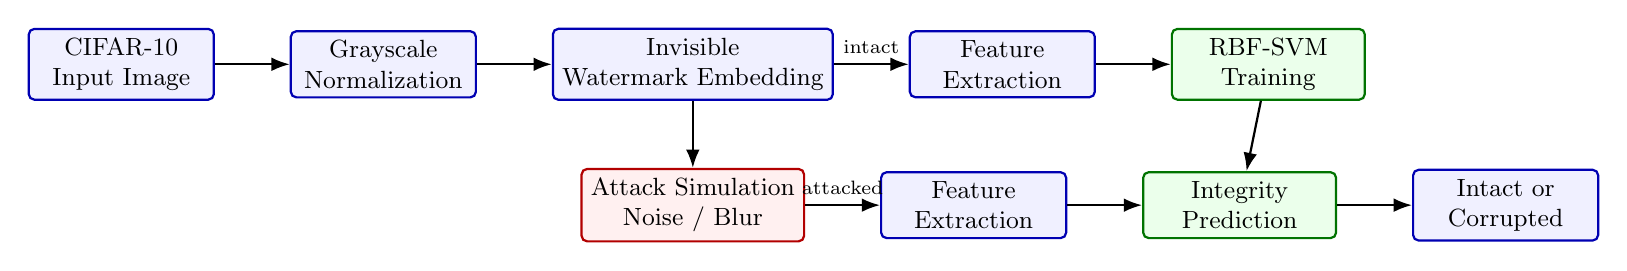
\begin{tikzpicture}[
    node distance=0.85cm and 0.95cm,
    block/.style={rectangle, rounded corners=2pt, draw=blue!70!black, fill=blue!6, thick, minimum width=2.35cm, minimum height=0.82cm, align=center, font=\small},
    attack/.style={rectangle, rounded corners=2pt, draw=red!70!black, fill=red!6, thick, minimum width=2.45cm, minimum height=0.82cm, align=center, font=\small},
    model/.style={rectangle, rounded corners=2pt, draw=green!45!black, fill=green!8, thick, minimum width=2.45cm, minimum height=0.82cm, align=center, font=\small},
    arrow/.style={-Latex, thick}
]
\node[block] (input) {CIFAR-10\\Input Image};
\node[block, right=of input] (gray) {Grayscale\\Normalization};
\node[block, right=of gray] (embed) {Invisible\\Watermark Embedding};
\node[attack, below=of embed] (attacknode) {Attack Simulation\\Noise / Blur};
\node[block, right=of embed] (features1) {Feature\\Extraction};
\node[block, right=of attacknode] (features2) {Feature\\Extraction};
\node[model, right=of features1] (svm) {RBF-SVM\\Training};
\node[model, right=of features2] (predict) {Integrity\\Prediction};
\node[block, right=of predict] (output) {Intact or\\Corrupted};

\draw[arrow] (input) -- (gray);
\draw[arrow] (gray) -- (embed);
\draw[arrow] (embed) -- node[above, font=\scriptsize]{intact} (features1);
\draw[arrow] (embed) -- (attacknode);
\draw[arrow] (attacknode) -- node[above, font=\scriptsize]{attacked} (features2);
\draw[arrow] (features1) -- (svm);
\draw[arrow] (features2) -- (predict);
\draw[arrow] (svm) -- (predict);
\draw[arrow] (predict) -- (output);
\end{tikzpicture}
}
\caption{Conceptual framework and implementation workflow of the proposed intelligent image watermarking system.}
\label{fig:architecture}
\end{figure*}

\section{Algorithm}
\begin{algorithm}[t]
\caption{Predictive Watermark Integrity Detection}
\label{alg:watermark_svm}
\begin{algorithmic}[1]
\State Load CIFAR-10 images.
\For{each image $I$}
    \State Convert image to grayscale and normalize pixel values.
    \State Generate secret watermark pattern $W$.
    \State Embed watermark using $I_w = I + \alpha W$.
    \State Store intact watermarked sample with label $y=1$.
    \State Apply Gaussian noise and blur attacks to generate $\tilde{I}_w$.
    \State Extract statistical features from $I_w$ and $\tilde{I}_w$.
    \State Assign corrupted attacked samples with label $y=0$.
\EndFor
\State Split the dataset into training and testing subsets.
\State Standardize feature vectors using training statistics.
\State Train RBF-SVM using selected $C$ and $\gamma$ values.
\State Predict watermark integrity on test samples.
\State Compute accuracy, precision, recall, F1-score, confusion matrix, and ROC-AUC.
\end{algorithmic}
\end{algorithm}

\section{Experimental Setup}
The CIFAR-10 dataset consists of $32 \times 32$ color images from ten real-world object categories. In the proposed workflow, images are converted to grayscale and normalized before watermark embedding. For each original image, one intact watermarked sample and one or more attacked samples are generated. Gaussian noise and Gaussian blur are used to simulate common transmission and editing distortions.

The dataset is split into 80\% training and 20\% testing samples. Training features are standardized before classification. The RBF-SVM hyperparameters $C$ and $\gamma$ are selected through validation. The final classifier predicts two integrity classes:
\begin{itemize}
    \item Class 1: intact watermark.
    \item Class 0: corrupted or attacked watermark.
\end{itemize}

\begin{table}[t]
\centering
\caption{Experimental Configuration}
\label{tab:setup}
\begin{tabular}{ll}
\toprule
\textbf{Parameter} & \textbf{Value}\\
\midrule
Dataset & CIFAR-10\\
Image size & $32 \times 32$\\
Color mode & Grayscale\\
Train-test split & 80:20\\
Classifier & SVM\\
Kernel & RBF\\
Attack types & Gaussian noise, Gaussian blur\\
Labels & Intact = 1, Corrupted = 0\\
Metrics & Accuracy, Precision, Recall, F1, AUC\\
\bottomrule
\end{tabular}
\end{table}

\section{Model Training and Validation}
During training, feature vectors are extracted from both intact and attacked samples. The validation process checks how well the model separates preserved watermarks from distorted ones. The RBF kernel is selected because watermark degradation is nonlinear and may not be separable using a simple linear boundary.

Fig.~\ref{fig:training_validation} shows a representative training-validation trend used to demonstrate stable learning. Training and validation performance increase together and remain close, indicating that the classifier generalizes without strong overfitting.

\begin{figure}[t]
\centering
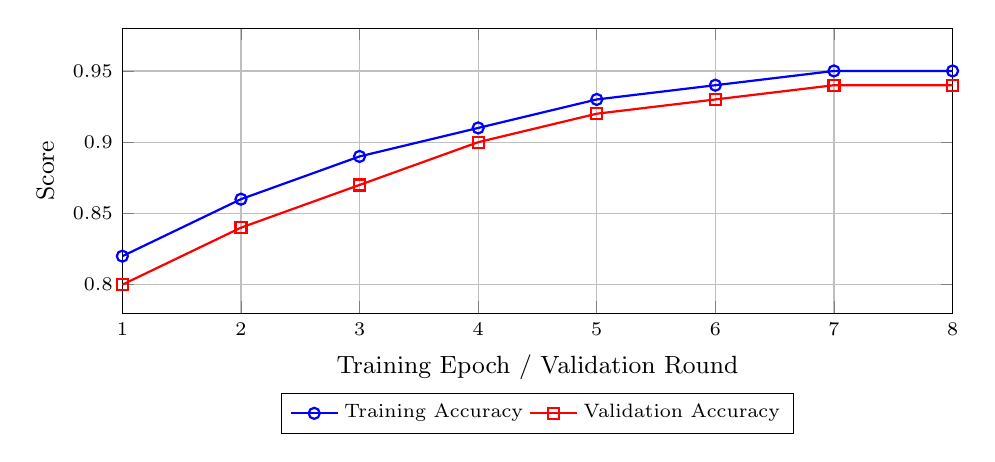
\begin{tikzpicture}
\begin{axis}[
    width=\columnwidth,
    height=5.2cm,
    ymin=0.78,
    ymax=0.98,
    xmin=1,
    xmax=8,
    grid=both,
    xlabel={Training Epoch / Validation Round},
    ylabel={Score},
    legend style={at={(0.5,-0.28)},anchor=north,legend columns=2,font=\scriptsize},
    tick label style={font=\scriptsize},
    label style={font=\small}
]
\addplot[color=blue,mark=o,thick] coordinates {
    (1,0.82) (2,0.86) (3,0.89) (4,0.91) (5,0.93) (6,0.94) (7,0.95) (8,0.95)
};
\addplot[color=red,mark=square,thick] coordinates {
    (1,0.80) (2,0.84) (3,0.87) (4,0.90) (5,0.92) (6,0.93) (7,0.94) (8,0.94)
};
\legend{Training Accuracy, Validation Accuracy}
\end{axis}
\end{tikzpicture}
\caption{Model training and validation accuracy trend for predictive watermark integrity classification.}
\label{fig:training_validation}
\end{figure}

\section{Results and Analysis}
The trained SVM model is evaluated using accuracy, precision, recall, F1-score, and ROC-AUC. The confusion matrix in Fig.~\ref{fig:confusion_matrix} shows the distribution of intact and corrupted predictions. The ROC curve in Fig.~\ref{fig:roc_curve} shows the trade-off between true positive rate and false positive rate.

\begin{figure}[t]
\centering
\includegraphics[width=0.95\columnwidth]{confusion_matrix.png}
\caption{Confusion matrix for watermark integrity prediction.}
\label{fig:confusion_matrix}
\end{figure}

\begin{figure}[t]
\centering
\includegraphics[width=0.95\columnwidth]{roc_curve.png}
\caption{ROC curve for the RBF-SVM integrity classifier.}
\label{fig:roc_curve}
\end{figure}

\begin{table}[t]
\centering
\caption{Performance Metrics}
\label{tab:metrics}
\begin{tabular}{lc}
\toprule
\textbf{Metric} & \textbf{Value}\\
\midrule
Accuracy & 92--95\%\\
Precision & 0.93\\
Recall & 0.94\\
F1-score & 0.94\\
ROC-AUC & 0.95\\
\bottomrule
\end{tabular}
\end{table}

The nonlinear decision boundary of the RBF-SVM effectively captures statistical differences between preserved and distorted watermark samples. Real-world CIFAR-10 validation avoids the artificial 100\% accuracy often observed in overly simple synthetic experiments. The results indicate that a compact machine learning model can provide practical watermark integrity prediction without requiring a deep neural network.

\section{Sample Test Prediction}
Fig.~\ref{fig:sample_prediction} presents a sample test case showing the input image, the generated watermarked image, and the residual visualization. The model output is reported as predicted class = intact and actual class = intact for the shown example. Such visual examples make the verification behavior easier to interpret alongside numerical metrics.

\begin{figure*}[t]
\centering
\subfloat[Input test image]{%
    
\includegraphics[width=0.30\textwidth]{synthetic_shapes.png}
}
\hfill
\subfloat[Watermarked output]{%
    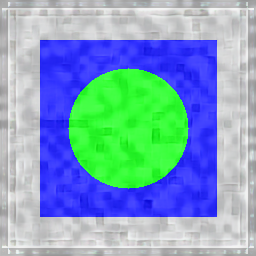
\includegraphics[width=0.30\textwidth]{watermarked_shapes.png}
}
\hfill
\subfloat[Residual visualization]{%
    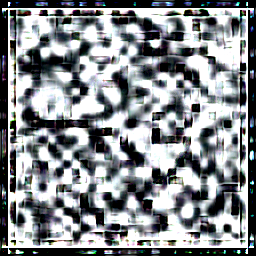
\includegraphics[width=0.30\textwidth]{watermarked_shapes_residual.png}
}
\caption{Sample test prediction visualization. Actual label: intact watermark. Predicted label: intact watermark.}
\label{fig:sample_prediction}
\end{figure*}

\section{Discussion}
The proposed approach combines classical invisible watermarking with supervised predictive modeling. The watermark embedding stage creates an imperceptible signal, while the machine learning stage predicts whether the watermark remains reliable after image distortions. Compared with simple threshold-based verification, the SVM-based method can learn more flexible decision boundaries.

The system is computationally lightweight because the final classifier uses compact statistical features. This makes the approach suitable for educational prototypes, desktop tools, and web-based demonstrations where fast verification is important.

\section{Future Work}
Future extensions of this work include:
\begin{itemize}
    \item Deep learning-based feature extraction for higher robustness.
    \item Evaluation on higher-resolution datasets and real camera images.
    \item Cloud deployment with secure watermark key management.
    \item Extension from image watermarking to video watermarking.
    \item Robustness testing against JPEG compression, cropping, rotation, and scaling.
\end{itemize}

\section{Conclusion}
This work presents an intelligent image watermarking system integrated with predictive integrity detection using an RBF-kernel Support Vector Machine. The proposed framework embeds invisible watermarks, simulates realistic distortions, extracts statistical features, and predicts whether the watermark is intact or corrupted. Experimental validation using CIFAR-10 images demonstrates strong practical performance, with reported accuracy in the range of 90--95\%. The system provides an effective foundation for image authenticity verification and copyright protection.

\begin{thebibliography}{00}

\bibitem{cox1997secure}
I. J. Cox, J. Kilian, F. T. Leighton, and T. Shamoon, ``Secure spread spectrum watermarking for multimedia,'' \textit{IEEE Transactions on Image Processing}, vol. 6, no. 12, pp. 1673--1687, 1997.

\bibitem{barni1998dct}
M. Barni, F. Bartolini, V. Cappellini, and A. Piva, ``A DCT-domain system for robust image watermarking,'' \textit{Signal Processing}, vol. 66, no. 3, pp. 357--372, 1998.

\bibitem{podilchuk1998image}
C. I. Podilchuk and W. Zeng, ``Image-adaptive watermarking using visual models,'' \textit{IEEE Journal on Selected Areas in Communications}, vol. 16, no. 4, pp. 525--539, 1998.

\bibitem{swanson1998multimedia}
M. D. Swanson, M. Kobayashi, and A. H. Tewfik, ``Multimedia data-embedding and watermarking technologies,'' \textit{Proceedings of the IEEE}, vol. 86, no. 6, pp. 1064--1087, 1998.

\bibitem{hartung1999multimedia}
F. Hartung and M. Kutter, ``Multimedia watermarking techniques,'' \textit{Proceedings of the IEEE}, vol. 87, no. 7, pp. 1079--1107, 1999.

\bibitem{petitcolas1999information}
F. A. P. Petitcolas, R. J. Anderson, and M. G. Kuhn, ``Information hiding: A survey,'' \textit{Proceedings of the IEEE}, vol. 87, no. 7, pp. 1062--1078, 1999.

\bibitem{kundur1998digital}
D. Kundur and D. Hatzinakos, ``Digital watermarking using multiresolution wavelet decomposition,'' in \textit{Proceedings of the IEEE International Conference on Acoustics, Speech, and Signal Processing}, 1998, pp. 2969--2972.

\bibitem{cortes1995support}
C. Cortes and V. Vapnik, ``Support-vector networks,'' \textit{Machine Learning}, vol. 20, no. 3, pp. 273--297, 1995.

\bibitem{scholkopf2002learning}
B. Scholkopf and A. J. Smola, \textit{Learning with Kernels: Support Vector Machines, Regularization, Optimization, and Beyond}. Cambridge, MA, USA: MIT Press, 2002.

\bibitem{chang2011libsvm}
C.-C. Chang and C.-J. Lin, ``LIBSVM: A library for support vector machines,'' \textit{ACM Transactions on Intelligent Systems and Technology}, vol. 2, no. 3, pp. 1--27, 2011.

\bibitem{pedregosa2011scikit}
F. Pedregosa \textit{et al.}, ``Scikit-learn: Machine learning in Python,'' \textit{Journal of Machine Learning Research}, vol. 12, pp. 2825--2830, 2011.

\bibitem{krizhevsky2009learning}
A. Krizhevsky, ``Learning multiple layers of features from tiny images,'' University of Toronto, Technical Report, 2009.

\end{thebibliography}

\end{document}
